\documentclass[12pt]{article}
\usepackage[utf8]{inputenc}
\usepackage[brazil]{babel}
\usepackage{graphicx}
\usepackage{amsmath}
\usepackage{listings}
\usepackage{color}
\usepackage{caption}
\usepackage{geometry}
\usepackage{float}  
\geometry{a4paper, margin=2.5cm}

\definecolor{codegray}{rgb}{0.5,0.5,0.5}
\definecolor{codepurple}{rgb}{0.58,0,0.82}

\lstset{
  language=[x86masm]Assembler,
  basicstyle=\ttfamily\footnotesize,
  keywordstyle=\color{blue},
  commentstyle=\color{codegray},
  stringstyle=\color{codepurple},
  numbers=left,
  numberstyle=\tiny\color{codegray},
  stepnumber=1,
  numbersep=5pt,
  showstringspaces=false,
  breaklines=true,
  breakatwhitespace=false,
  tabsize=2
}

\title{Projeto de Processador REDUX-V}
\author{Pietro Comin - GRR20241955}
\date{\today}

\begin{document}

\maketitle

\begin{abstract}
Este relatório documenta o projeto do processador REDUX-V, abordando sua arquitetura, conjunto de instruções, componentes principais como a ULA e a memória de controle, além da justificativa para instruções estendidas adicionadas. 
\end{abstract}

\section{Introdução}

Este relatório apresenta o desenvolvimento completo da arquitetura REDUX-V, uma arquitetura de 8 bits do tipo load-store, com organização monociclo e endereçamento por byte. O projeto foi implementado no Logisim Evolution, utilizando memória RAM do tipo \texttt{dual\_port\_ram}, e com clock de dois ticks por ciclo. 

Por praticidade e facilidade nos testes, foram adicionadas duas memórias ROM dentro do componente \texttt{dual\_port\_ram}, que contêm o hexadecimal das instruções de ambos os trabalhos desenvolvidos até então na disciplina. Na implementação do código, o fato de haver uma ou duas unidades de memória não é importante, pois somente são armazenados dados na RAM a partir do endereço final das instruções contidas na ROM.

Além das instruções da arquitetura base, foram implementadas três novas instruções utilizando opcodes reservados: \texttt{jien}, \texttt{muli} e \texttt{brzrue}. Estas instruções, que serão melhor detalhadas mais à frente, visam ampliar a flexibilidade do programa de teste, com destaque para saltos condicionais estendidos e multiplicação com imediato.

\section{Conjunto de Instruções Base}

A arquitetura REDUX-V suporta um conjunto enxuto de instruções, como:

\begin{itemize}
  \item Operações lógicas: \texttt{and}, \texttt{or}, \texttt{not}, \texttt{xor}
  \item Operações aritméticas: \texttt{add}, \texttt{sub}, \texttt{addi}, \texttt{slr}, \texttt{srr}
  \item Controle de fluxo: \texttt{ji} (jump immediate), \texttt{brzr} (branch if zero)
  \item Manipulação de registradores e memória: \texttt{load}, \texttt{store}
\end{itemize}

\section{Datapath do Processador}

\begin{figure}[H]
\centering
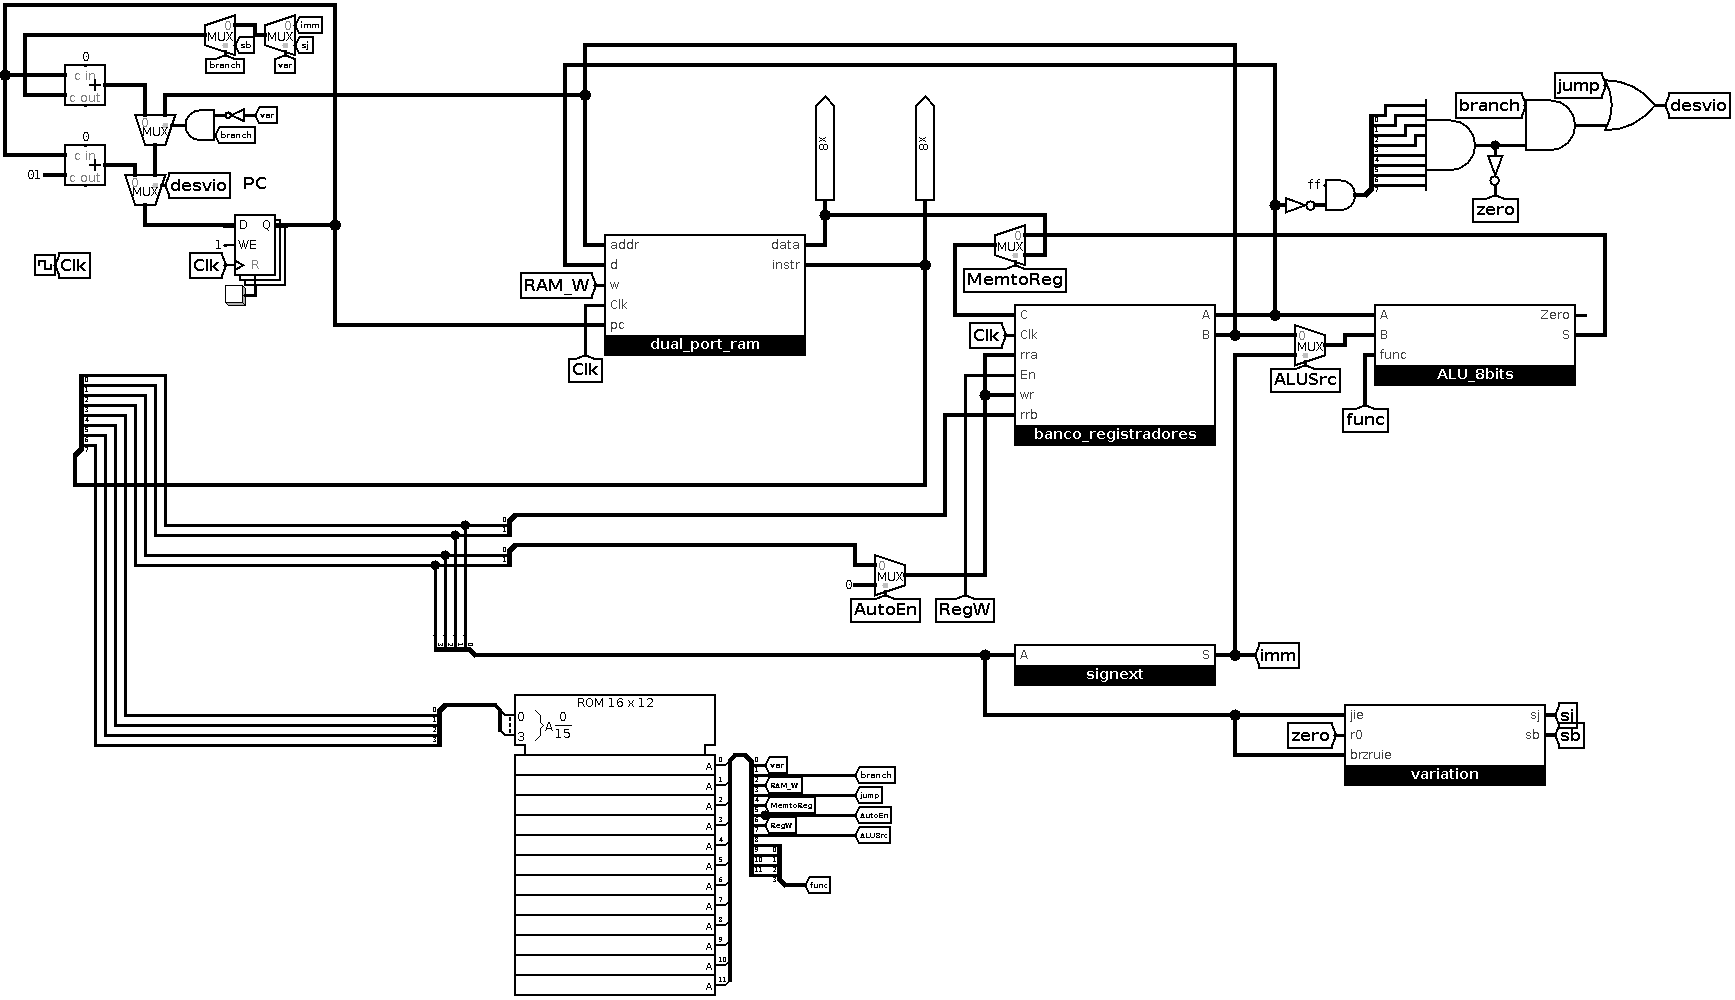
\includegraphics[width=0.9\textwidth]{/images/Redux-V_datapath.png}
\caption{Datapath do processador REDUX-V}
\label{fig:datapath}
\end{figure}

O datapath define o caminho de dados percorrido durante a execução de uma instrução. Ele inclui componentes como o banco de registradores, a ULA, multiplexadores, unidade de controle, extensor de sinal, componente de variação nos saltos e memória de dados.

\section{Projeto da ULA}

\begin{figure}[H]
\centering
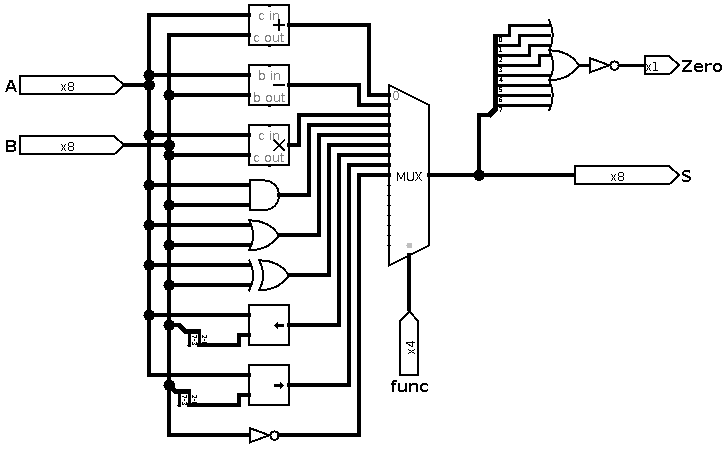
\includegraphics[width=0.75\textwidth]{/images/ALU.png}
\caption{Diagrama interno da ULA}
\label{fig:ula}
\end{figure}

A ULA é responsável por executar as operações lógicas, aritméticas e de deslocamento da arquitetura REDUX-V. Ela recebe dois operandos e um código de operação (func), realizando o processamento e enviando o resultado ao banco de registradores ou à memória.

\subsection{Operações Suportadas}
\begin{itemize}
  \item Operações lógicas: \texttt{not}, \texttt{and}, \texttt{or}, \texttt{xor}
  \item Operações aritméticas: \texttt{add}, \texttt{sub}, \texttt{addi}, \texttt{muli}
  \item Deslocamentos: \texttt{slr}, \texttt{srr}
  \item Comparações: implícitas no controle de fluxo (\texttt{brzr})
\end{itemize}

\subsection{Controle da ULA}
O código de operação que define o comportamento da ULA é fornecido pela memória de controle, a partir do opcode decodificado da instrução atual.

\section{Memória de Controle}

A memória de controle foi projetada para fornecer os sinais necessários à execução de cada instrução, com base no opcode correspondente. Ela determina os sinais de controle para os multiplexadores, leitura e escrita de registradores, operação da ULA e controle de fluxo (como atualização do PC).

\begin{figure}[H]
\centering
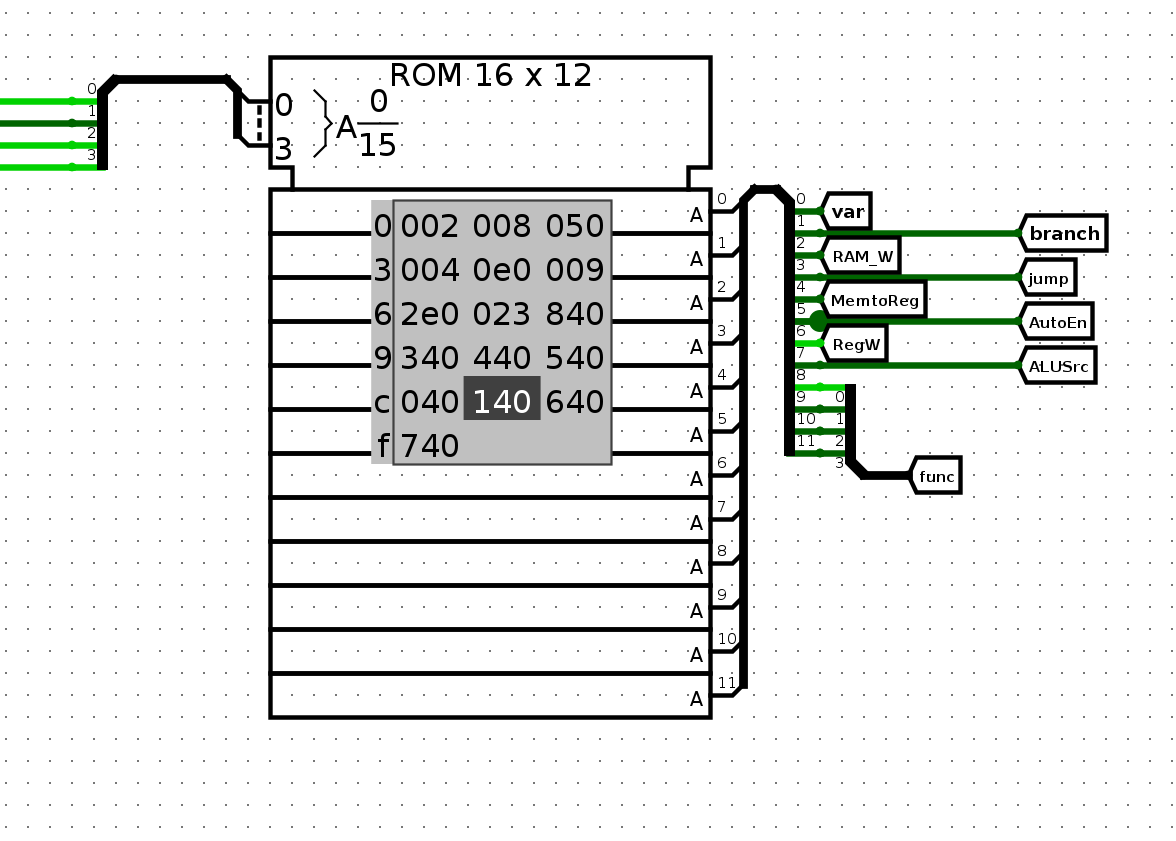
\includegraphics[width=0.85\textwidth]{/images/controll_memory.png}
\caption{Diagrama da memória de controle do processador REDUX-V}
\label{fig:memoria_controle}
\end{figure}

\section{Justificativa das Instruções Adicionais}

As três instruções estendidas adicionadas à arquitetura (\texttt{jien}, \texttt{muli} e \texttt{brzrue}) visam ampliar a capacidade da linguagem de máquina e tornar os programas mais enxutos e expressivos.

\begin{itemize}
  \item \textbf{jien} (Jump Immediate Extended Negative): permite saltos para trás mais longos do que o \texttt{ji}. Ideal para loops e estruturas de repetição. É uma instrução do tipo I que recebe um imediato, multiplica-o por dois, soma 9 e retorna o resultado negativo em B+1. A soma com 9 acontece pois o range de um imediato de 4 bits é [-8, 7], então a instrução é otimizada.

  \textit{Adendo: A instrução \texttt{jien} foi primeiramente implementada com a ideia de permitir um salto positivo ou negativo, dependendo do conteúdo de \texttt{r[0]}. Se seu conteúdo fosse igual a 0, o salto seria positivo; caso contrário, negativo. Contudo, para melhor usabilidade no código de teste, a instrução foi modificada para sempre realizar um salto negativo. O circuito anterior foi mantido, mas encontra-se inoperante.}

  \item \textbf{muli} (Multiplication Immediate): substitui múltiplas instruções \texttt{addi} por uma única operação de multiplicação com imediato. Como são reservados somente 4 bits de imediato, é difícil atingir valores grandes usando poucas instruções e com mais precisão que usar um shift. Por isso muli foi implementado.
  \item \textbf{brzrue} (Branch on Zero Unsigned Extended): permite saltos condicionais longos para frente, o que facilita implementações mais complexas com bifurcações. Também uma instrução do tipo I, recebe um imediato, multiplica-o por dois e soma 8.
\end{itemize}

\begin{figure}[H]
\centering
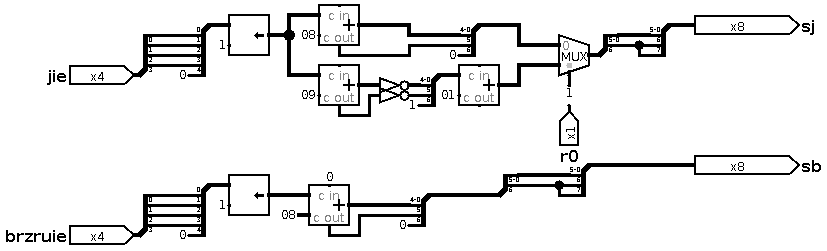
\includegraphics[width=0.65\textwidth]{/images/variation_component.png}
\caption{Componente de variação utilizado no cálculo de endereço das instruções \texttt{jien} e \texttt{brzrue}}
\label{fig:variation}
\end{figure}

\subsection{Exemplo de Código com Instruções Estendidas}

\begin{lstlisting}
; Programa que calcula um valor, aplica salto positivo e negativo
loop:
brzrue 2      ; PC = PC + 12 (se r[0] == 0, salta para fim_loop)
... (11 instrucoes)
jien 1        ; PC = PC - 11 (salto para loop)

fim_loop:
...
\end{lstlisting}

Essas instruções contribuem para a legibilidade e eficiência do código Assembly por aumentar o range dos saltos e tirar a necessidade de cálculo manual do endereço de destino do PC.

\section{Assembly}

\subsection{Trabalho 1}
\begin{lstlisting}
sub r0, r0
sub r1, r1
sub r2, r2  
sub r3, r3   

; os vetores comecarao no endereco de memoria 110

; inicia valores 
addi 1
sub r3, r0      ; r3 = -1
addi 7
addi 2          ; r0 = 10
sub r1, r0      ; r1 = -10
add r0, r0      ; r0 = 20
add r0, r0      ; r0 = 40
addi 5          ; r0 = 45
addi 5          ; r0 = 50
add r2, r0      ; r2 = 50
sub r0, r1      ; r0 = 60
st r0, r3       ; 60 armazenado em 0xff
add r3, r3      ; r3 = -2
add r2, r2      ; r2 = 100
sub r2, r1      ; r2 = 110
st r2, r3       ; 110 armazenado em 0xfe
sub r0, r0
sub r2, r2
sub r3, r3


; calcula o fim_loop (PC = 23)
addi 1
sub r3, r3
sub r3, r0      ; end = -1
ld r3, r3       ; end = fim_loop
sub r0, r0

loop:
brzr r1, r3
; ajusta i 
addi 7          ; r0 = 7
addi 3          ; r0 = 10
add r1, r0      ; i += 10
; guarda 1 
sub r0, r0      ; r0 = 0
addi 2          ; r0 = 2
sub r3, r3
sub r3, r0      ; end = -2
ld r3, r3       ; end = 110
add r3, r1      ; end = 110 + deslocamento (i)
sub r0, r0      ; r0 = 0
st r2, r3       ; M[end] = x
; guarda 2 
addi 1          ; r0 = 1
add r2, r0      ; x += 1
addi 7          ; r0 = 8
addi 2          ; r0 = 10
add r3, r0      ; end = 110 + deslocamento + 10
st r2, r3       ; M[end] = x
; ajusta parametros para reiniciar loop 
sub r0, r0
addi 7
addi 2          ; r0 = 9
sub r1, r0      ; i -= 9
addi 1          ; r0 = 10
add r0, r0      ; r0 = 20
addi 3          ; r0 = 23
sub r3, r3      ; end = 0
add r3, r0      ; end = 23
sub r0, r0      ; r0 = 0
addi 1          ; r0 = 1
add r2, r0      ; x += 1
sub r0, r0      ; r0 = 0
brzr r0, r3     ; forca o salto para PC = 23

fim_loop:



; soma dos vetores

sub r2, r2      ; PC = 60
sub r3, r3
addi 7
addi 3          ; r0 = 10
sub r1, r0      ; i = -10
sub r0, r0

; calcula r3 (PC = 66) 
sub r3, r3
addi 2          ; r0 = 2
sub r3, r0      ; r3 = -2
ld r3, r3       ; r3 = 110
addi 2          ; r0 = 4
sub r3, r0      ; r3 = 106
sub r0, r0

loop_2:
brzr r1, r3
addi 7
addi 3          ; r0 = 10
add r1, r0      ; i += 10
;
sub r0, r0
sub r3, r3
addi 2          ; r0 = 2
sub r3, r0      ; r3 = -2
ld r3, r3       ; r3 = 110
add r3, r1      ; r3 += deslocamento (i)
ld r2, r3       ; r2 = M[end]
addi 7          ; r0 = 9
addi 1          ; r0 = 10
add r3, r0      ; r3 += 10
ld r0, r3       ; r0 = M[r3]
add r2, r0      ; soma dos vetores
sub r0, r0
addi 7
addi 3          ; r0 = 10
add r3, r0      ; r3 += 10
st r2, r3       ; M[end] = r2
sub r0, r0      ; r0 = 0
;
addi 7
addi 2          ; r0 = 9
sub r1, r0      ; i -= 9
addi 7          ; r0 = 16
add r0, r0      ; r0 = 32
add r0, r0      ; r0 = 64
addi 2          ; r0 = 66
sub r3, r3
add r3, r0      ; r3 = 66
sub r0, r0
brzr r0, r3


fim_loop_2:
addi 3          ; PC = 106
add r3, r0      ; r3 = 109
sub r0, r0
ji 0            ; halt (PC = PC + 0)

\end{lstlisting}

\subsection{Trabalho 2}

\begin{lstlisting}

sub r0, r0
sub r1, r1
sub r2, r2  
sub r3, r3   

; os vetores comecarao no endereco de memoria 72

; inicia valores 
addi 7
addi 3          ; r0 = 10
sub r1, r0      ; r1 = -10
muli 7          ; r0 = 70
addi 2          ; r0 = 72
add r3, r0      ; r3 = 72
sub r2, r2
sub r0, r0
add r0, r1      ; r0 = i      

loop:
brzruie 8       ; 8 * 2 + 8
; ajusta i 
sub r0, r0
addi 7          ; r0 = 7
addi 3          ; r0 = 10
add r1, r0      ; i += 10
; guarda 1 
sub r0, r0      ; r0 = 0
add r3, r1      ; end = base + deslocamento (i)
st r2, r3       ; M[end] = x
; guarda 2 
addi 1          ; r0 = 1
add r2, r0      ; x += 1
addi 7          ; r0 = 8
addi 2          ; r0 = 10
add r3, r0      ; end = base + deslocamento + 10
st r2, r3       ; M[end] = x
sub r3, r1      ; r3 = base + 10
sub r3, r0      ; r3 = base
; ajusta parametros para reiniciar loop 
addi -1         ; r0 = 9
sub r1, r0      ; i -= 9
sub r0, r0      ; r0 = 0
addi 1          ; r0 = 1
add r2, r0      ; x += 1
sub r0, r0      ; r0 = 0
add r0, r1      ; se i = 0 saira do loop
jie 8           ; -(8 * 2 + 7)

fim_loop:



; soma dos vetores

sub r2, r2
addi 7
addi 3          ; r0 = 10
sub r1, r0      ; i = -10
sub r0, r0
add r0, r1      ; r0 = i
or r0, r0       ; jump pula para ca

loop_2:
brzruie 9       ; PC = 44
sub r0, r0      ; r0 = 0
addi 7
addi 3          ; r0 = 10
add r1, r0      ; i += 10
;
sub r0, r0
add r3, r1      ; r3 += deslocamento (i)
ld r2, r3       ; r2 = M[end]
addi 7          ; r0 = 7
addi 3          ; r0 = 10
add r3, r0      ; r3 = base + 10
ld r0, r3       ; r0 = M[end]
add r2, r0      ; soma dos vetores
sub r0, r0
addi 7
addi 3          ; r0 = 10
add r3, r0      ; r3 = base + 10
st r2, r3       ; M[end] = r2
sub r3, r1
sub r3, r0
sub r3, r0      ; r3 = base
;
addi -1         ; r0 = 9
sub r1, r0      ; i -= 9
sub r0, r0
add r0, r1      ; r0 = i
jien 8          ; PC = 68


fim_loop_2:
or r0, r0
ji 0            ; halt (PC = PC + 0)

\end{lstlisting}

\section{Conclusão}

O projeto do processador REDUX-V evidenciou os princípios fundamentais da arquitetura de computadores, incluindo o funcionamento de uma ULA, memória de controle e fluxo de dados via datapath. As instruções adicionais propostas aumentaram a flexibilidade da linguagem e a expressividade dos programas escritos para essa arquitetura.

\end{document}

